\ProvidesClass{twentysecondcv}[2015/02/28 CV class]
\LoadClass{article}
\NeedsTeXFormat{LaTeX2e}

%----------------------------------------------------------------------------------------
%	 REQUIRED PACKAGES
%-----------------------------------------------------------------------	-----------------

\RequirePackage[quiet]{fontspec}
\RequirePackage[sfdefault]{ClearSans}

\def\arrow#1{\pspicture[shift=2pt](#1,0)\psline{->}(#1,0)\endpspicture}

\usepackage{pstricks}

\usepackage{fontawesome}
\RequirePackage{tikz}
\RequirePackage{xcolor}
\RequirePackage[absolute,overlay]{textpos}
\RequirePackage{ragged2e}
\RequirePackage{etoolbox}
\RequirePackage{ifmtarg}
\RequirePackage{ifthen}
\RequirePackage{pgffor}
\RequirePackage{marvosym}
\RequirePackage{parskip}

\usepackage{enumitem}
\setlist[itemize]{leftmargin=*}

\RequirePackage[hidelinks]{hyperref}
\hypersetup{
    pdftitle={},
    pdfauthor={},
    pdfsubject={},
    pdfkeywords={},
    colorlinks=false,           % no lik border color
    allbordercolors=white       % white border color for all
}

\DeclareOption*{\PassOptionsToClass{\CurrentOption}{article}}
\ProcessOptions\relax

\ifxetex
  \usepackage{letltxmacro}
  \setlength{\XeTeXLinkMargin}{1pt}
  \LetLtxMacro\SavedIncludeGraphics\includegraphics
  \def\includegraphics#1#{% #1 catches optional stuff (star/opt. arg.)
    \IncludeGraphicsAux{#1}%
  }%
  \newcommand*{\IncludeGraphicsAux}[2]{%
    \XeTeXLinkBox{%
      \SavedIncludeGraphics#1{#2}%
    }%
  }%
\fi

%----------------------------------------------------------------------------------------
%	 COLOURS
%----------------------------------------------------------------------------------------

\definecolor{white}{RGB}{255,255,255}
\definecolor{gray}{HTML}{4D4D4D}
\definecolor{sidecolor}{HTML}{E7E7E7}
\definecolor{mainblue}{HTML}{0E5484}
\definecolor{maingray}{HTML}{B9B9B9}

\definecolor{pblue}{HTML}{0395DE}

\definecolor{darkgray}{HTML}{333333}
\definecolor{gray}{HTML}{4D4D4D}
\definecolor{lightgray}{HTML}{999999}
\definecolor{green}{HTML}{C2E15F}
\definecolor{orange}{HTML}{FDA333}
\definecolor{purple}{HTML}{D3A4F9}
\definecolor{red}{HTML}{FB4485}
\definecolor{blue}{HTML}{6CE0F1}
\definecolor{pblue}{HTML}{0395DE}
\definecolor{materialpurple}{HTML}{9C27B0}
\definecolor{materialindigo}{HTML}{3F51B5}
\definecolor{materialblue}{HTML}{2196F3}
\definecolor{materialcyan}{HTML}{00BCD4}
\definecolor{materialteal}{HTML}{009688}
\definecolor{materialgreen}{HTML}{4CAF50}
\definecolor{materiallime}{HTML}{CDDC39}
\definecolor{materialamber}{HTML}{FFC107}
\definecolor{materialbrown}{HTML}{795548}
\definecolor{materialred}{HTML}{FF4436}
\definecolor{materialorange}{HTML}{FF5722}
\definecolor{linkedin}{HTML}{0085AE}
\definecolor{test}{HTML}{0077be}
\definecolor{yt}{HTML}{c71610}
\definecolor{darkblue}{HTML}{353747}
\ifdefined\@cv@print
  \colorlet{green}{gray}
  \colorlet{orange}{gray}
  \colorlet{purple}{gray}
  \colorlet{red}{gray}
  \colorlet{blue}{gray}
  \colorlet{fillheader}{white}
  \colorlet{header}{gray}
\else
  \colorlet{fillheader}{white}
  \colorlet{header}{gray}
\fi
\colorlet{textcolor}{gray}
\colorlet{headercolor}{darkblue}


%----------------------------------------------------------------------------------------
%	 MISC CONFIGURATIONS
%----------------------------------------------------------------------------------------

% \renewcommand{\bfseries}{\color{black}} % Make \textbf produce coloured text instead

\pagestyle{empty} % Disable headers and footers

\setlength{\parindent}{0pt} % Disable paragraph indentation

% --------------------------------------------------------------------------------------
% 	FONTS
%-------------------------------------------------------------------------------------
\newfontfamily\headingfont[Path = fonts/]{segoeuib.ttf}

%----------------------------------------------------------------------------------------
%	 SIDEBAR DEFINITIONS
%----------------------------------------------------------------------------------------

\setlength{\TPHorizModule}{1cm} % Left margin
\setlength{\TPVertModule}{1cm} % Top margin

\newlength\imagewidth
\newlength\imagescale
\pgfmathsetlength{\imagewidth}{5cm}
\pgfmathsetlength{\imagescale}{\imagewidth/600}

\newcommand{\profilesection}[2]{\vspace{8pt}{\color{black!80} \huge #1 \rule[0.15\baselineskip]{#2}{1pt}}}

% Define custom commands for CV info
\newcommand{\cvdate}[1]{\renewcommand{\cvdate}{#1}}
\newcommand{\cvlinkedin}[1]{\renewcommand{\cvlinkedin}{#1}}
\newcommand{\cvgithub}[1]{\renewcommand{\cvgithub}{#1}}
\newcommand{\cvmail}[1]{\renewcommand{\cvmail}{#1}}
\newcommand{\cvnumberphone}[1]{\renewcommand{\cvnumberphone}{#1}}
\newcommand{\cvaddress}[1]{\renewcommand{\cvaddress}{#1}}
\newcommand{\cvsite}[1]{\renewcommand{\cvsite}{#1}}
\newcommand{\aboutme}[1]{\renewcommand{\aboutme}{#1}}
\newcommand{\profilepic}[1]{\renewcommand{\profilepic}{#1}}
\newcommand{\cvname}[1]{\renewcommand{\cvname}{#1}}
\newcommand{\cvjobtitle}[1]{\renewcommand{\cvjobtitle}{#1}}
\newcommand{\cvnationality}[1]{\renewcommand{\cvnationality}{#1}}
% \newcommand{\cvnationality}[1]{\renewcommand{\cvnationality}{#1}}

% Command for printing the contact information icons
\newcommand*\icon[1]{\tikz[baseline=(char.base)]{\node[shape=circle,draw,inner sep=1pt, fill=mainblue,mainblue,text=white] (char) {#1};}}

% Command for printing skill progress bars
\newcommand\programming[1]{ 
	\renewcommand{\programming}{
		\begin{tikzpicture}
        % 	\node [above right] at (0, 4) {$0 \: LOC \: \arrow{3.2} \: 5000 \: LOC$};
			\foreach [count=\i] \x/\y in {#1}{
				% \draw[fill=maingray,maingray] (0,\i) rectangle (6,\i+0.4);
				% \draw[fill=white,mainblue](0,\i) rectangle (\y,\i+0.4);
			 %   \filldraw[black] (0,0) circle (2pt) node[anchor=south] {$(4.2,5.9)$};
			     \node [above right] at (0,\i+0.5+0.35) {\textbf{\y}};
				\node [above right] at (0,\i+0.35) {\x};
			}
		\end{tikzpicture}
	}
}

\newcommand\lang[1]{ 
	\renewcommand{\lang}{
		\begin{tikzpicture}
        % 	\node [above right] at (0, 4) {$0 \: LOC \: \arrow{3.2} \: 5000 \: LOC$};
			\foreach [count=\i] \x/\y in {#1}{
				% \draw[fill=maingray,maingray] (0,\i) rectangle (6,\i+0.4);
				% \draw[fill=white,mainblue](0,\i) rectangle (\y,\i+0.4);
			 %   \filldraw[black] (0,0) circle (2pt) node[anchor=south] {$(4.2,5.9)$};
			     \node [above right] at (0,\i+0.5+0.35) {\textbf{\y}};
				\node [above right] at (0,\i+0.35) {\x};
			}
		\end{tikzpicture}
	}
}

\newcommand\projects[1]{ 
	\renewcommand{\projects}{
		{#1}
	}
}

\newcommand\tools[1]{ 
	\renewcommand{\tools}{
		{#1}
	}
}
\newcommand\concepts[1]{ 
	\renewcommand{\concepts}{
		{#1}
	}
}

%----------------------------------------------------------------------------------------
%  SIDEBAR LAYOUT
%----------------------------------------------------------------------------------------

\newcommand{\makeprofile}{
  \begin{tikzpicture}[remember picture,overlay]
      \node [rectangle, fill=sidecolor, anchor=north, minimum width=9cm, minimum height=\paperheight+1cm] (box) at (-5cm,0.5cm){};
  \end{tikzpicture}

  %------------------------------------------------

  \begin{textblock}{6}(0.5, 0.2)

    %------------------------------------------------
    \begin{center}
        {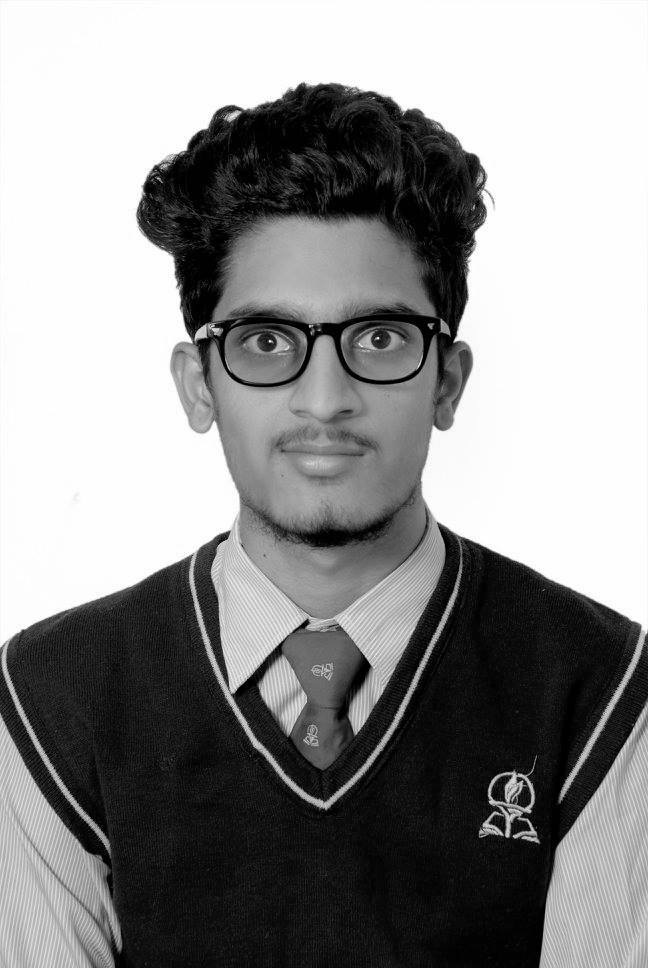
\includegraphics[width=80mm,height=50mm,clip,keepaspectratio]{Rohit_CV-v1/rohitimg.jpg}}
    \end{center}
    
    
    %------------------------------------------------
        \vspace{4mm}
    {\Huge\color{pblue}\cvname}
    \vspace{2mm}

    %------------------------------------------------
    
    % {\Large\color{black!80}\cvjobtitle}
    \vspace{-3mm}
    %------------------------------------------------
    {\Medium\color{black!80}\cvnationality} 
    

    
    \vspace{-1mm}
    {\Medium\color{black!90}\cvaddress}
    %------------------------------------------------
    
    \vspace{3mm}
    \renewcommand{\arraystretch}{2}
    \begin{tabular}{p{1cm} @{\hskip 0.5cm}p{5cm}}
      \ifthenelse{\equal{\cvnumberphone}{}}{}{
      		{$
              \begin{array}{l}
              \hspace{4mm} \Huge \textnormal{\faMobile} 
              \end{array}
              $} 
            & \cvnumberphone\\}
            
    %   \ifthenelse{\equal{\href{\cvsite}{\cvsite}}{}}{}{
    %         {$
    %           \begin{array}{l}
    %           \hspace{2.8mm} \huge \textnormal{\textcolor{test}{\faGlobe}}
    %           \end{array}
    %           $} 
    %         & \href{http://\cvsite}{\cvsite} \\}
      \ifthenelse{\equal{\cvmail}{}}{}{
            {$
              \begin{array}{l}
              \hspace{2.5mm} \huge \textnormal{\textcolor{yt}{\faEnvelopeO}}
              \end{array}
              $} 
            & \href{mailto:\cvmail}{\cvmail} \\}
      
        
        \ifthenelse{\equal{\cvgithub}{}}{}{
            {$
              \begin{array}{l}
              \hspace{3mm} \huge \textnormal{\faGithub}
              \end{array}
              $} & \href{https://www.github.com/\cvgithub}{\cvgithub} \\
            }   
        \ifthenelse{\equal{\cvlinkedin}{}}{}{
            {$
              \begin{array}{l}
              \hspace{3mm} \huge \textnormal{\textcolor{linkedin}{\faLinkedin}}
              \end{array}
              $} & \href{https://www.linkedin.com/in/\cvlinkedin}{\cvlinkedin} \\
            }    
    \end{tabular}

    %------------------------------------------------
    \vspace{2mm}
    % \profilesection{Skills}{4cm}
    
    % {\large \textbf{Overview}}

% 	\skills
        
        %------------------------------------------------
        
        %\vspace{2mm}
       
% 	 {\large \textbf{Programming}} 
        \profilesection{Programming}{1.55cm} 
		 \programming
		 \vspace{2mm}\\ \\
          \profilesection{Languages}{2.5cm} 
		 \lang
		
        \vspace{1mm}
        \\
        % \profilesection{Projects}{3cm} 
        
        %  \projects
          \profilesection{Concepts }{2.5cm} 
        
            \concepts
        \profilesection{Tools }{4cm} 
        
            \tools
        
  \end{textblock}
}


%----------------------------------------------------------------------------------------
%	 COLOURED SECTION TITLE BOX
%----------------------------------------------------------------------------------------

% Command to create the rounded boxes around the first three letters of section titles
\newcommand*\round[2]{%
	\tikz[baseline=(char.base)]\node[anchor=north west, draw,rectangle, rounded corners, inner sep=1.6pt, minimum size=5.5mm, text height=3.6mm, fill=#2,#2,text=white](char){#1};%
}

\def\@sectioncolor#1#2#3{%
	{%
	       %  #1#2#3
		 #1#2#3%
	}%
}


\renewcommand{\section}[1]{
  \par\vspace{\parskip}
	{%
		\LARGE\headingfont\color{headercolor}%
		\@sectioncolor #1%
	}
  \par\vspace{\parskip}
}

\renewcommand{\subsection}[1]{
	\par\vspace{.5\parskip}{%
		\Large\headingfont\color{headercolor} #1%
	}
	\par\vspace{.25\parskip}%
}

\pagestyle{empty}

%----------------------------------------------------------------------------------------
%	 LONG LIST ENVIRONMENT
%----------------------------------------------------------------------------------------

\setlength{\tabcolsep}{0pt}

% New environment for the long list
\newenvironment{twenty}{%
	\begin{tabular*}{\textwidth}{@{\extracolsep{\fill}}ll}
}{%
	\end{tabular*}
}

% \newcommand{\twentyitem}[5]{%
% 	#1&\parbox[t]{0.83\textwidth}{%
% 		\textbf{#2}% 
% 		\hfill%
% 		{\footnotesize#3}\\%
%         \ifblank{#4}{}{#4 \\}
% 		#5\vspace{\parsep}%
% 	}\\
% }

\newcommand{\twentyitem}[6]{%
	#1&\parbox[t]{0.83\textwidth}{%
		\textbf{#3}% 
		\hfill%
		{\footnotesize#4}%
        }\\%
    #2&\parbox[t]{0.83\textwidth}{%
		\ifblank{#5}{}{#5 \\}
		#6%
	}\\
}

%----------------------------------------------------------------------------------------
%	 SMALL LIST ENVIRONMENT
%----------------------------------------------------------------------------------------

\setlength{\tabcolsep}{0pt}

% New environment for the small list
\newenvironment{twentyshort}{%
	\begin{tabular*}{\textwidth}{@{\extracolsep{\fill}}ll}
}{%
	\end{tabular*}
}

\newcommand{\twentyitemshort}[2]{%
	#1&\parbox[t]{0.83\textwidth}{%
		#2%
	}\\
}

%----------------------------------------------------------------------------------------
%	 MARGINS AND LINKS
%----------------------------------------------------------------------------------------

\RequirePackage[left=7.6cm,top=0.1cm,right=1cm,bottom=0.1cm,nohead,nofoot]{geometry}


\usepackage{smartdiagram}
\smartdiagramset{
    bubble center node font = \footnotesize,
    bubble node font = \footnotesize,
    % specifies the minimum size of the bubble center node
    bubble center node size = 0.5cm,
    %  specifies the minimum size of the bubbles
    bubble node size = 0.5cm,
    % specifies which is the distance among the bubble center node and the other bubbles
    distance center/other bubbles = 0.3cm,
    % sets the distance from the text to the border of the bubble center node
    distance text center bubble = 0.5cm,
    % set center bubble color
    bubble center node color = pblue,
    % define the list of colors usable in the diagram
    set color list = {lightgray, materialcyan, orange, green, materialorange, materialteal, materialamber, materialindigo, materialgreen, materiallime},
    % sets the opacity at which the bubbles are shown
    bubble fill opacity = 0.6,
    % sets the opacity at which the bubble text is shown
    bubble text opacity = 1,
}

